
\chapter{Introduction}
This thesis considers the problem of tracking human wrist movements during free living. This is motivated by the fact that wrist and hand movements can be used detect periods of eating~\cite{dong2013detecting} and then further track the amount of food that is being ingested by a person~\cite{dong2012new}. Eating can occur at any time of the day, and it very hard to monitor the activity as such. We propose a solution which uses a wrist watch like device to monitor how the wrist is moving throughout the day, and store it on a memory chip.
\section{Motivation}
\label{Sec:Motivation}

 Obesity is an increasing problem. CDC (Centers for Disease Control and Prevention) reports mention one
 \textemdash{} third of the adult American population as 
 obese, while sixty nine percent of the population is considered 
 overweight. The CDC defines individuals with a Body Mass
 Index of twenty five and above as overweight~\cite{ogden2010prevalence}.
 This number is rising in children too, with eighteen
 percent children between the ages of 12 \textemdash{} 18
 years considered obese. Modern advances have helped our minds work
 on autopilot. Not only is it easy to order food, but consuming
 food while watching television or using a computer makes
 it very easy to consume a large amount of calories quickly without
 noticing it happen. when a group
 of individuals was asked to count the number of bites taken over
 a 24 hour period, 40\% lost count or forgot entirely ~\cite{mahoney1975obese}.
 The abundance of fast food chains, high calorie food, and soda dispensers makes it very easy
 for a person to consume a large amount of calories without realizing 
 that they are doing so. Children who ate fast food, compared with those who did not,
 consumed an average of 187 kcal more every day ~\cite{bowman2004effects}.
 Eating slowly is shown to help decrease the amount of calories
 consumed during a meal~\cite{Andrade2008}, however it is not an
 easy change to make in our busy lives.

\begin{figure}
\begin{center}
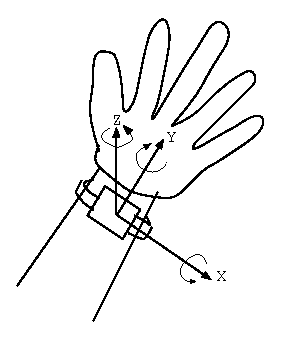
\includegraphics{images/HandAxis.eps}
\caption{A wrist watch shaped device showing the different axis being recorded.}
\label{fig:HandAxis}
\end{center}
\end{figure}
 
 
\section{Fitness Tracking}
\label{Sec:FitnessTracking}
\begin{figure}
%\begin{center}
\centering
\begin{subfigure}[b]{0.4\textwidth}
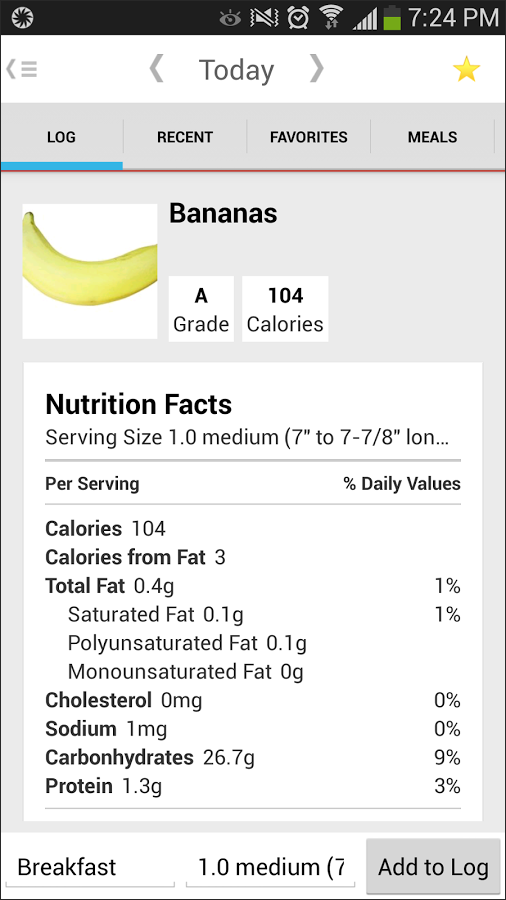
\includegraphics[width=0.8\textwidth]{images/CCScreenshot.PNG}
\caption{Calorie Counter}
\label{fig:CCScreenshot}
\end{subfigure}
\qquad
\begin{subfigure}[b]{0.4\textwidth}
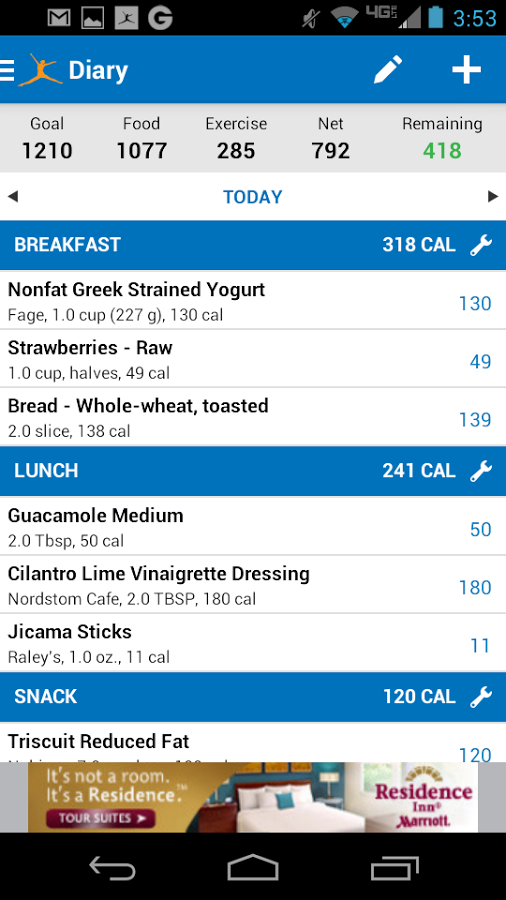
\includegraphics[width=0.8\textwidth]{images/MyFitScreenshot.png}
\caption{MyFitnessPal}
\label{fig:MyFitScreenshot}
\end{subfigure}
\caption{Screenshots of two famous Fitness Tracking Software}
\label{fig:FitnessScreenshots}
%\end{center}
\end{figure}
With the increase in smart phone sales, we see a huge rise in small applications that help track our daily activities. Applications like CalorieCount\footnote{Allows users to name and record calories consumed. Users can pick from a database or enter their own values.} and MyFintessPal\footnote{Allows users to pick various foods or exercises from a database or enter their own data.} allow users to track their daily intake of food and also track other activities like exercise and sleep. However, this data was still largely dependent on the user's ability to record these events.
Smaller sensors and components have allowed wearable devices to enter the market. These devices are a part of clothing or accessories  that contain a microcomputer to perform electronic functions, and can have a battery life of 24 to 48 hours.

\begin{figure}
\begin{center}
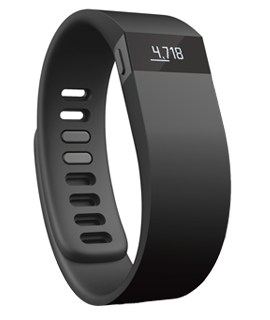
\includegraphics[width=0.8\textwidth]{images/JawFit.png}
\caption{The Fitbit flex (left) and the Jawbone Up activity trackers}
\label{fig:FitbitJawbone}

\end{center}
\end{figure}
Fitness trackers in the market currently offer a range of services. The Fitbit\footnote{http://www.fitbit.com} and Jawbone\footnote{http://www.jawbone.com} series of sensors allow for exercise and sleep monitoring using wrist movements. This data is then synchronized with a computer or a mobile phone, and can be viewed graphically by the user. Another consumer electronic segment that has now emerged is smart watches. These watches contain electronic components that make them functionally similar to a mobile phone, and are small enough to wear on the wrist. They contain low power displays and have a host of power saving techniques to have a long battery life. However most of the wearable devices on are limited to counting the number of calories expended and thus not many options exist for counting the number of calories consumed.
\section{Wearable Wrist Motion Tracker}
\label{Sec:WearbleTracker}
Work done in \cite{drennan2010assessment} shows a device that is capable of detecting bites by monitoring wrist movement
We are motivated by the problem of monitoring calorie consumption by creating a wrist watch like device that automates the process. Since the device is to be worn by the user everyday, it needs to have a small size. To avoid having to recharge often, or risking the battery dying during a meal, the device also needs to have a good battery life\footnote{Requiring a recharge not more than once a day}. Our device records raw inertial movement data (Rotation and Acceleration), and stores this in a memory chip. The configuration of the various axes is displayed in Figure \ref{fig:HandAxis}.
The data can later be accessed later using a computer and can processed by algorithms shown in ~\cite{dong2012new} to show when a bite of food has been eaten.

\section{Previous Work}

\section{Shimmer}